% Toolbar icon: beam — a slender member drawn as a tube, with its circular
% cross-section shown end-on. That pairing is the whole point of the feature:
% a line cell alone has no extent, and it is the SECTION (Kratos CROSS_AREA,
% kept in the mdpa Properties block) that turns it into drawable geometry.
\documentclass[tikz,border=2mm]{standalone}
\usetikzlibrary{arrows.meta,calc,shapes.geometric}
\begin{document}
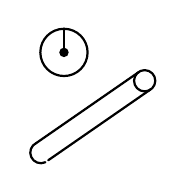
\begin{tikzpicture}[line width=1.3pt, line cap=round, line join=round, x=1mm,y=1mm]
  % The tube: two parallel sides running down-left to up-right, closed at the
  % far end by an ellipse read as the section seen at a glancing angle.
  \draw[thick] (-8,-5.5) -- (5,3.5);
  \draw[thick] (-6.5,-7.7) -- (6.5,1.3);
  % Near end cap.
  \draw[thick] (-8,-5.5) arc (115:295:1.35 and 1.35);
  % Far end cap, drawn whole so the section reads as a circle.
  \draw[thick] (5.75,2.4) circle (1.35);
  % The section called out: a small circle with its radius, set apart from the
  % member so it reads as the property rather than as more geometry.
  \draw[thick] (-4.5,6) circle (3);
  \draw[thick] (-4.5,6) -- (-4.5,9);
  \fill (-4.5,6) circle (0.6);
\end{tikzpicture}
\end{document}
